\documentclass[11pt,a4paper]{article}
\usepackage[T1]{fontenc}
\usepackage[utf8]{inputenc}
\usepackage{lmodern,microtype}
\usepackage[margin=25mm]{geometry}
\usepackage{amsmath,amssymb}
\usepackage{graphicx,booktabs,tabularx,array}
\usepackage{caption,xspace,xcolor}
\usepackage[numbers,sort&compress]{natbib}
\usepackage[hyphens]{url}
\usepackage[colorlinks=true,linkcolor=black,citecolor=black,urlcolor=blue]{hyperref}
\usepackage{fancyhdr,placeins,listings,float}
\hypersetup{pdftitle={Missile Intercept: A Contract-Driven Multi-Rate Framework for Reproducible Flight Simulation},pdfauthor={Anonymous Authors}}
\definecolor{codebg}{HTML}{F4F6F8}
\captionsetup{font=small,labelfont=bf}
\setlength{\parskip}{3pt}
\setlength{\parindent}{1.2em}
\setlength{\emergencystretch}{2em}
\clubpenalty=10000
\widowpenalty=10000
\pagestyle{fancy}
\fancyhf{}
\fancyhead[L]{\small\textit{Contract-Driven Multi-Rate Flight Simulation}}
\fancyhead[R]{\small Anonymous preprint}
\fancyfoot[C]{\thepage}
\renewcommand{\headrulewidth}{0.3pt}
\setlength{\headheight}{14pt}
\lstset{basicstyle=\small\ttfamily,columns=fullflexible,keepspaces=true,breaklines=true,breakatwhitespace=true,showstringspaces=false,backgroundcolor=\color{codebg},frame=single,rulecolor=\color{black!15},framesep=6pt,aboveskip=10pt,belowskip=10pt}
% Fresh verification results generated on 2026-11-14.
\newcommand{\NumericalCases}{5\xspace}
\newcommand{\NumericalFailed}{0\xspace}
\newcommand{\ApplicationTestsPassed}{83\xspace}
\newcommand{\ApplicationTestsFailed}{0\xspace}

\newcommand{\code}[1]{\texttt{#1}}
\newcolumntype{Y}{>{\raggedright\arraybackslash}X}
\newcolumntype{P}[1]{>{\raggedright\arraybackslash}p{#1}}

\title{\vspace{-1em}\textbf{Missile Intercept: A Contract-Driven Multi-Rate\\Framework for Reproducible Flight Simulation}}
\author{Anonymous Authors}
\date{November 14, 2026}

\begin{document}
\maketitle
\thispagestyle{plain}
\begin{abstract}
End-to-end flight simulation must couple continuous dynamics, sampled sensors, decision modules, actuator commands, event handling, and experiment records without allowing their timing or data conventions to drift apart. Existing research codes often provide either easily modified component models or tightly integrated scenario scripts, but leave the sampled-data semantics, array layout, and provenance of reported outputs implicit. This paper presents \emph{Missile Intercept}, a Python framework organized around three mechanisms: a deterministic multi-rate closed-loop architecture, contract-driven state and telemetry interfaces, and a layered verification and traceability workflow. Discrete modules are sampled on explicit clocks and held through fixed-step Runge--Kutta stages; event refinement preserves the outer sampling grid. Metadata-bearing schemas derive contiguous state layouts and stable layout identifiers, while bounded telemetry makes admission, ownership, and export behavior explicit. Verification combines manufactured numerical problems, orbital and quaternion invariants, cross-integrator checks, interface probes, and application tests. In a fresh execution, all five numerical verification cases and all 83 automated tests pass. These results establish the implemented software and numerical contracts, not physical or operational validity. The framework thereby turns a monolithic scenario workflow into an inspectable research instrument whose execution semantics, exchanged data, and evidence chain can be reproduced and extended.
\end{abstract}
\noindent\textbf{Keywords:} flight simulation; sampled-data systems; multi-rate integration; software architecture; verification; reproducibility

\section{Introduction}
High-dynamic flight research depends on simulation long before a complete experimental system exists. A useful simulator must represent the vehicle and environment, synthesize observations, execute decision and command logic, integrate continuous dynamics, identify events, and retain enough intermediate state to explain an outcome. These concerns operate on different time scales and through different representations. Consequently, a credible end-to-end result depends not only on a physical model, but also on software decisions about when modules run, which values remain frozen during integration, how state fields map into arrays, and which execution produced a figure.

Component-oriented scientific codes make individual models easy to inspect, yet their composition frequently relies on informal conventions. A sensor may expect one coordinate frame while the dynamics expose another; a controller may be called inside every Runge--Kutta stage even though it represents sampled hardware; or an array offset may change without invalidating downstream post-processing. At the other extreme, a monolithic scenario script can hide these inconsistencies behind a single entry point. The resulting program may produce plots while remaining difficult to test, modify, or compare.

Software and benchmark papers suggest complementary remedies. Stable-Baselines3 couples a common interface with tested reference implementations \citep{raffin2021}; CleanRL makes implementation and experimental records directly inspectable \citep{huang2022}; and OpenML benchmarking suites treat tasks, protocols, and run records as first-class objects \citep{bischl2021}. In flight dynamics, JSBSim illustrates the value of a reusable software boundary around a simulation engine \citep{berndt2026}. These systems differ from the present application, but they share a principle: scientific claims become easier to assess when execution semantics and evidence are explicit.

The original \emph{Missile Intercept} archive contains a six-degree-of-freedom flight simulation organized into environment, vehicle, sensing, estimation, decision, command, numerical, and reporting modules. Its earlier description emphasized inventory and report provenance. That framing did not explain the central technical problem---the composition of continuous and sampled subsystems---and did not show how the implementation enforces the required contracts. This paper therefore recasts the archive as a software and numerical-method contribution. It describes implementation mechanisms at the level needed to reproduce the behavior, while deliberately omitting operational design guidance and treating historical report pages with missing execution provenance as unverified artifacts.

The objective is to provide an inspectable end-to-end research framework in which timing, representation, and evidence remain aligned. The contributions are:
\begin{enumerate}
  \item a \emph{deterministic multi-rate closed-loop architecture} that separates continuous dynamics from sampled modules, applies zero-order holds through the Runge--Kutta stages, and refines events without shifting the controller sample grid;
  \item a \emph{contract-driven state and telemetry interface} that derives contiguous storage from named metadata, records layout identity, validates boundary conditions, and states copy/view and capacity semantics; and
  \item a \emph{layered verification and traceability workflow} joining analytic numerical tests, invariant and cross-integrator checks, interface probes, application tests, seeded batch execution, and machine-readable evidence.
\end{enumerate}
The remainder of the paper follows the problem--method--evidence chain. Section~2 defines the end-to-end composition problem and its difficulties. Section~3 presents the three implementation mechanisms. Section~4 reports numerical, interface, and application-level verification. Section~5 concludes with the supported claims, limitations, and next steps.

\section{Problem Formulation}
Let the continuous plant state be $x(t)\in\mathbb{R}^{n}$ and let $z_i[k]$ denote the internal state of discrete module $i$ at its $k$th release. A closed-loop research simulation can be written as
\begin{align}
\dot{x}(t) &= f\!\left(t,x(t),u(t),w(t)\right), \\
z_i[k+1] &= F_i\!\left(z_i[k],y_i(t_{i,k}),\theta_i\right), \\
u(t) &= H\!\left(z_1[k_1(t)],\ldots,z_m[k_m(t)]\right),
\end{align}
where $w$ represents the modeled environment, $y_i$ is the input observed by module $i$, $t_{i,k}$ is its sampling time, and $\theta_i$ is its configuration. The experiment additionally produces a record $r_j=(t_j,q_j)$ at logging times $t_j$, where $q_j$ contains named diagnostic quantities. The implementation problem is to advance these coupled states while preserving each module's clock, the meaning of every exchanged field, and the history required to interpret the resulting records.

Three difficulties dominate. The first is \emph{timing ambiguity}. If sampled sensors and control modules are evaluated inside the four stages of a classical RK4 step, their internal states can advance several times within what should be one hardware sample. If an event divides an integration step and the scheduler restarts at the event, later sample times can shift. Both errors change the discrete system even when the continuous right-hand side is unchanged. Adaptive integration introduces a related ambiguity because rejected trial steps must not trigger irreversible sampled-data updates.

The second difficulty is \emph{representation drift}. Numerical kernels prefer contiguous arrays, while component authors reason about names, shapes, units, frames, and ownership. Hand-written offsets make this translation brittle. Runtime types alone are insufficient: a Python array does not state whether it is a copy or a view, which frame it uses, or whether an added field changed the serialized layout. Telemetry creates a second representation boundary in which capacity, timestamp ordering, nonfinite values, and decimal export must have defined behavior.

The third difficulty is \emph{evidence fragmentation}. Unit tests, numerical checks, batch runs, plots, and HTML reports often live in separate directories without a common execution record. A deterministic solver cannot make an experiment reproducible if its configuration, seed, environment, or source version is unknown. Conversely, a source hash taken today cannot reconstruct the provenance of an older plot. Reproducible research therefore requires both executable checks and honest limits on what their records establish \citep{sandve2013,barba2021}.

These difficulties rule out a simple ``one script, one time step, one CSV'' design. The required solution must (i) define sampled-data semantics independently of the continuous integrator, (ii) make data layouts and ownership machine-checkable, and (iii) connect claims to fresh, retained verification records. Figure~\ref{fig:architecture} summarizes the resulting design.

\begin{figure}[t]
\centering
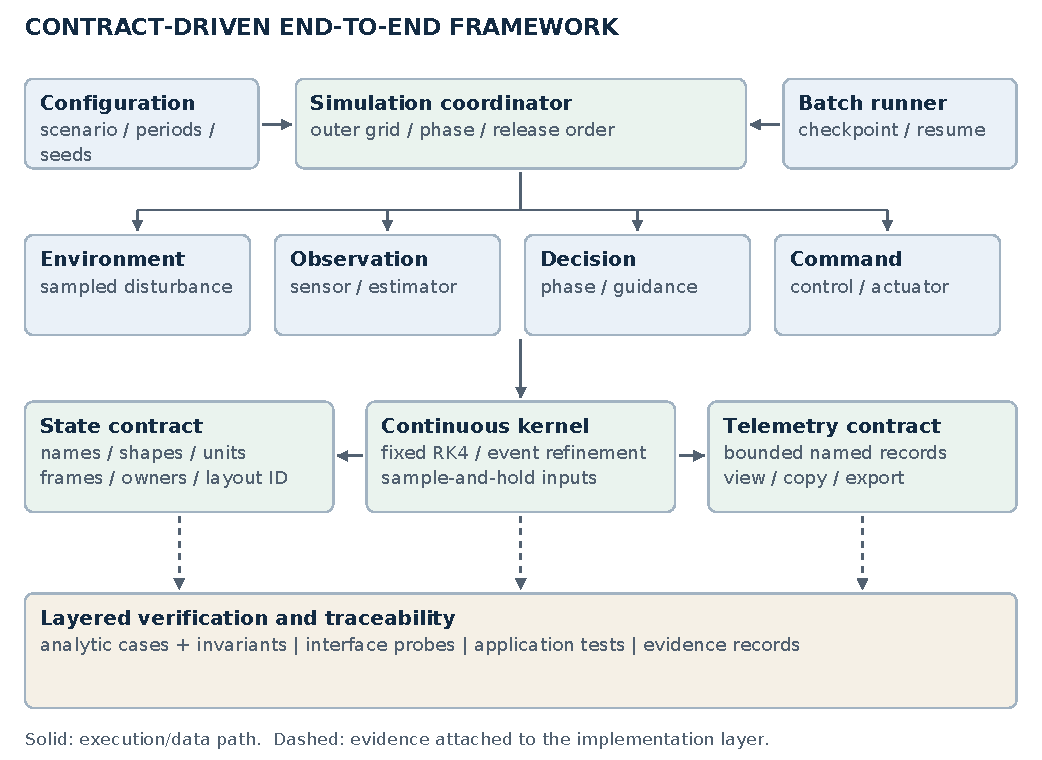
\includegraphics[width=\linewidth]{figures/framework_architecture.pdf}
\caption{End-to-end framework architecture. The coordinator owns the clocks and phase-independent execution order. Named contracts mediate between component objects and contiguous numerical state. Verification and traceability are cross-cutting rather than downstream presentation steps.}
\label{fig:architecture}
\end{figure}

\section{Method}
The framework applies the same three-part structure to every run. The deterministic multi-rate closed-loop architecture defines \emph{when} state may change. The contract-driven state and telemetry interface defines \emph{what} may cross a boundary and who owns it. The layered verification and traceability workflow defines \emph{which evidence} supports a claim. Together they separate domain models from the execution rules that make those models composable.

\subsection{Deterministic multi-rate closed-loop architecture}
\label{sec:multirate}
The central \code{Simulation} object composes configuration, state schema, environment and vehicle models, sampled components, an integrator, and a telemetry recorder. The continuous right-hand side is a pure evaluation of the current continuous state and values already frozen by the outer loop. Sampled sensors, estimation, decision, command, and actuator updates occur only in the \code{before\_step} callback. State projection and accepted-step bookkeeping occur in \code{after\_step}. This separation prevents RK4's internal stages from becoming unintended module releases.

Each periodic module uses a \code{MultiRateScheduler}. For period $T_i$ and next release $\tau_i$, module $i$ is due when $t+\epsilon \geq \tau_i$, where $\epsilon$ is a small comparison tolerance. After a release, the scheduler advances by integer periods until $\tau_i>t+\epsilon$. Advancing the stored deadline, rather than assigning $t+T_i$, avoids accumulating phase error when floating-point times lie slightly beyond a nominal release. The default configuration exposes separate periods for fast sampled modules, navigation updates, and logging, while the outer step can change by flight phase. These values are configuration, not hard-coded call-site delays.

At outer time $t_n$, the execution order is: sample the modeled environment; release every due observation module; update due decision and command modules; freeze their outputs; evaluate the continuous model through the four RK4 stages; project constrained state; and record due telemetry. If $h_n$ is the accepted outer interval and $u_n$ is the frozen command, the continuous update is
\begin{align}
k_1 &= f(t_n,x_n,u_n),\\
k_2 &= f(t_n+h_n/2,x_n+h_nk_1/2,u_n),\\
k_3 &= f(t_n+h_n/2,x_n+h_nk_2/2,u_n),\\
k_4 &= f(t_n+h_n,x_n+h_nk_3,u_n),\\
x_{n+1} &= \Pi\!\left[x_n+\frac{h_n}{6}(k_1+2k_2+2k_3+k_4)\right],
\end{align}
where $\Pi$ is an optional state projector. The same $u_n$ appears in every stage. Figure~\ref{fig:timeline} makes this hold semantics explicit.

\begin{figure}[t]
\centering
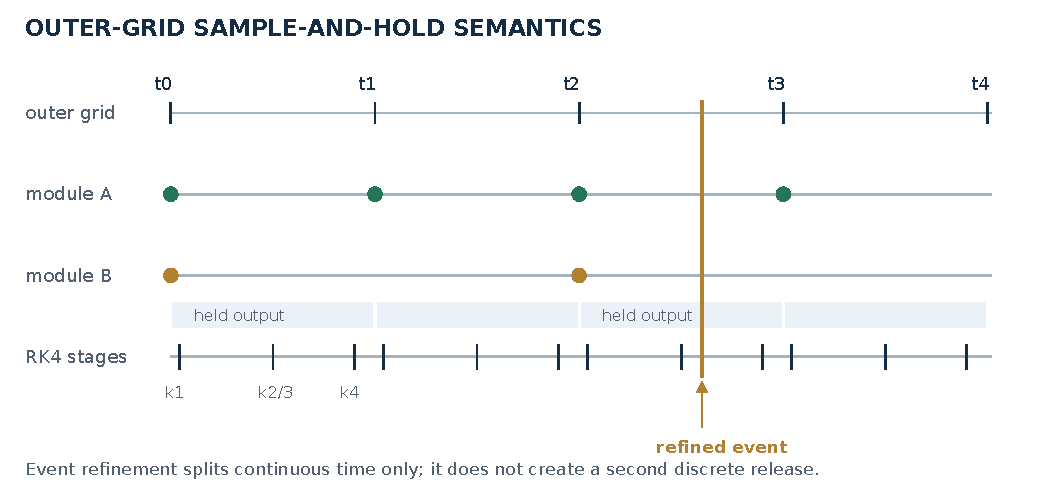
\includegraphics[width=\linewidth]{figures/multirate_timeline.pdf}
\caption{Sample-and-hold semantics. Due discrete modules execute once at an outer-grid release; their outputs remain fixed during all RK4 stages. An event may split the accepted continuous interval, but the discrete sample deadline remains anchored to the original outer grid.}
\label{fig:timeline}
\end{figure}

Events are represented by scalar guard functions with terminal and direction attributes. A sign change inside an accepted RK4 interval triggers bisection; each midpoint state is reconstructed by RK4 from the left bracket. Multiple roots within the tolerance are grouped. Crucially, a nonterminal event may divide the continuous interval, but it does not call \code{before\_step} again before the original \code{outer\_end}. This preserves the controller grid and the frozen values. The adaptive Cash--Karp RK45 path is restricted to continuous-only problems: the implementation rejects sampled callbacks and events instead of silently assigning them ambiguous rejection semantics.

The architecture is modular above this timing kernel. Component families exchange typed records and can be replaced within the same coordinator. The current archive contains phase management and several model families, but the paper's contribution is the execution contract rather than any particular domain-specific decision law. The expected effect is deterministic composition: identical configuration, source, and random seeds produce the same release sequence and numerical path on the same supported environment.

\subsection{Contract-driven state and telemetry interface}
\label{sec:contracts}
The numerical state boundary is specified by \code{StateField} and \code{StateSchema}. Each field has a key, shape, unit label, frame label, and owner. For ordered fields $i=1,\ldots,K$ with flattened sizes $d_i$, the schema derives
\begin{equation}
D=\sum_{i=1}^{K}d_i, \qquad s_i=\left[\sum_{j<i}d_j,\ \sum_{j\leq i}d_j\right).
\end{equation}
Thus one definition produces the total dimension $D$, the named slice $s_i$, packing order, unpacking shape, and metadata record. Duplicate keys are rejected at construction. A layout identifier hashes the ordered metadata serialization, so changes to names, shapes, units, frames, owners, or ordering are observable even if the total dimension remains constant.

\code{pack(mapping)} requires the exact key set, checks each declared shape, converts scalar fields by element count, writes a newly allocated floating-point vector, and rejects nonfinite packed values. \code{unpack(vector)} checks the total shape and returns Python scalars or copied arrays. Copying is intentional: a component receiving an unpacked field cannot mutate the solver state by aliasing it. Figure~\ref{fig:contracts} shows how metadata becomes contiguous storage and how the layout identifier protects the interface between source and retained artifacts.

\begin{figure}[t]
\centering
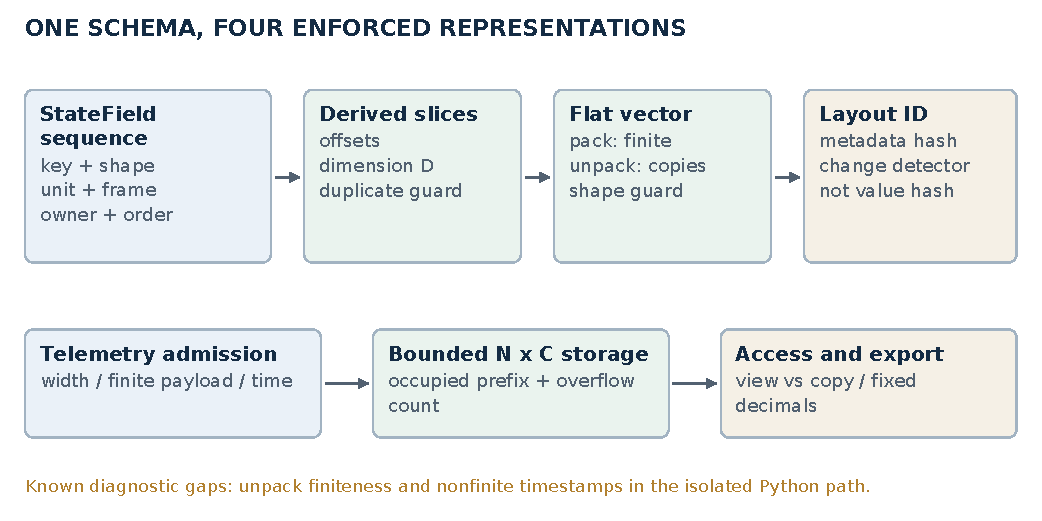
\includegraphics[width=\linewidth]{figures/data_contracts.pdf}
\caption{Contract-driven representation. One ordered schema generates named slices, packing and unpacking behavior, and a metadata layout identifier. The identifier covers representation metadata, not numerical values or physical correctness.}
\label{fig:contracts}
\end{figure}

Telemetry applies a parallel contract. \code{TelemetryLogger} preallocates an $N\times C$ float64 matrix, including time, and records the occupied prefix $n$. A call to \code{send(t,v)} checks payload width and finiteness, then returns a Boolean indicating admission. A full buffer increments an overflow counter; a non-increasing timestamp is rejected without changing the occupied prefix. The primary payload is predictably $B_{\mathrm{array}}=8NC$ bytes, excluding Python objects and copies. \code{get(name)} returns a storage-sharing column view, whereas \code{as\_dict()} returns copies. CSV export writes only accepted rows with a named header and fixed decimal formatting. These distinctions are part of the API because silent aliasing, silent row loss, or precision assumptions can invalidate downstream analysis.

The implementation does not claim a perfect formal type system. Dataclass annotations are inspectable but do not enforce all runtime types; \code{unpack} checks shape but not finiteness; and the isolated Python telemetry path validates payload values but does not reject a nonfinite timestamp. These boundaries are reported rather than hidden. The expected effect of the contract layer is earlier localization of integration errors and a stable, inspectable bridge between component-level reasoning and array-level numerical code.

\subsection{Layered verification and traceability workflow}
\label{sec:traceability}
The evidence workflow has four layers. First, analytic and invariant-based numerical cases test the integrator independently of the application. Second, interface probes exercise state and telemetry contracts with dimensionless synthetic records. Third, the application test suite checks scheduling, events, data consistency, component integration, and end-to-end smoke behavior. Fourth, artifact records retain the environment, source inventory, test reports, figures, and build checks used by this paper. A claim is included only when at least one retained record addresses it at the appropriate layer.

Batch execution derives a case seed from a base seed and case identifier, so scheduling order does not define the random stream. Each completed case can be appended to a JSON Lines checkpoint; resume mode loads completed case identifiers and schedules the remainder. This mechanism improves repeatability and failure recovery. It does not make results comparable unless configuration, code, and environment are also retained.

Traceability uses machine-readable records rather than relying on filenames alone. The paper package includes numerical-verification JSON, pytest JUnit XML, interface-probe JSON, source inventories, figure-generation code, LaTeX sources, and PDF checks. File digests can establish that a retained byte sequence matches an inventory, consistent with standard provenance concepts \citep{moreau2013,nist2015}; they cannot recover the execution history of a pre-existing report. Accordingly, all historical HTML results without report-specific manifests remain labeled \code{legacy\_unverified} and are excluded from the quantitative conclusions.

The three mechanisms form a closed reasoning chain: the multi-rate architecture defines execution, the contracts define exchanged data, and the workflow checks and records both. Their expected combined effect is not higher simulated performance, but lower ambiguity: a researcher can identify when a module ran, how a value was represented, and which executable check supports a stated software property.

\section{Simulation and Verification}
The evaluation asks three questions corresponding to the method. Does the numerical core display its expected behavior on problems with known answers or invariants? Do the state and telemetry boundaries enforce their documented contracts? Does the assembled application preserve those behaviors across its automated test surface and produce a self-contained paper artifact? The fresh run used the repository's existing Python environment; commands and machine-readable outputs are retained with the manuscript. No historical interception metric is used as a validation target.

\subsection{Numerical verification of the multi-rate core}
Five built-in cases exercise complementary numerical properties. The manufactured problem $\dot{y}=y$ integrates over successively refined fixed grids; the observed order is the minimum of adjacent error-ratio estimates. A two-body circular orbit tests relative radius and specific-energy conservation over one revolution. A long constant-rate attitude propagation checks quaternion normalization with the production projector. A fixed RK4 solution is compared with the continuous-only adaptive RK45 backend. Finally, RK45 position is compared with the analytic circular-orbit endpoint. Table~\ref{tab:numerical} reports the exact retained observations and acceptance limits.

\begin{table}[H]
\caption{Fresh built-in numerical verification. ``Observed'' is defined by each case and is compared with the stated one-sided acceptance condition.}
\label{tab:numerical}
\centering\small
\begin{tabularx}{\linewidth}{@{}Yrrl@{}}
\toprule
Case & Observed & Limit & Condition \\
\midrule
RK4 manufactured convergence order & 3.880 & 3.800 & $\geq$ \\
Kepler radius conservation (relative) & $7.959\times10^{-13}$ & $10^{-6}$ & $\leq$ \\
Quaternion norm deviation & $0$ & $10^{-12}$ & $\leq$ \\
RK4--RK45 relative position difference & $1.457\times10^{-9}$ & $10^{-8}$ & $\leq$ \\
Adaptive RK45 analytic position error & $4.561\times10^{-9}$ & $10^{-8}$ & $\leq$ \\
\bottomrule
\end{tabularx}
\end{table}

All \NumericalCases cases pass. The RK4 order approaches the theoretical fourth order, while the conservation and cross-method errors remain well below their thresholds. These tests support the fixed-step implementation, projection path, and continuous-only adaptive reference. They do not measure the accuracy of any aerodynamic, atmospheric, sensor, or decision model.

Scheduler and event semantics are tested at the software level. Cases cover due-time advancement, zero-order holding through RK4 stages, direction-aware guards, terminal and nonterminal roots, simultaneous events, tolerance handling, and the rule that event splitting does not resample discrete modules. The adaptive backend's rejection of sampled callbacks is also exercised. These are the failure modes most directly associated with the deterministic multi-rate closed-loop architecture.

\subsection{Verification of state and telemetry contracts}
The generic interface harness selects \code{StateField}, \code{StateSchema}, and \code{TelemetryLogger} from their source files and supplies a controlled namespace without importing the physical simulation. It exercises valid round trips, duplicate and missing keys, shape mismatches, nonfinite values, layout-identifier changes, view/copy ownership, timestamp ordering, capacity overflow, and CSV precision. This isolation makes failures attributable to the interface rather than to application setup.

Twenty-one of 23 targeted interface properties are observed. The two unmet stronger requirements are diagnostically useful: a correctly shaped nonfinite vector is accepted by \code{unpack}, and a NaN timestamp with finite payload is accepted in the isolated Python telemetry path. These are not converted into passes or removed from the record. Twelve allocation cases covering four capacities and three column counts match $8NC$ exactly. The result supports the stated layout, ownership, admission, and payload claims while identifying two guards for future strengthening.

Figure~\ref{fig:verification} maps evidence layers to claims. The structure intentionally avoids a single aggregate ``accuracy'' score: numerical convergence, interface enforcement, application integration, and artifact integrity answer different questions. This follows the same separation of implementation and experiment records that makes scientific software easier to inspect \citep{wilson2017,huang2022}.

\begin{figure}[H]
\centering
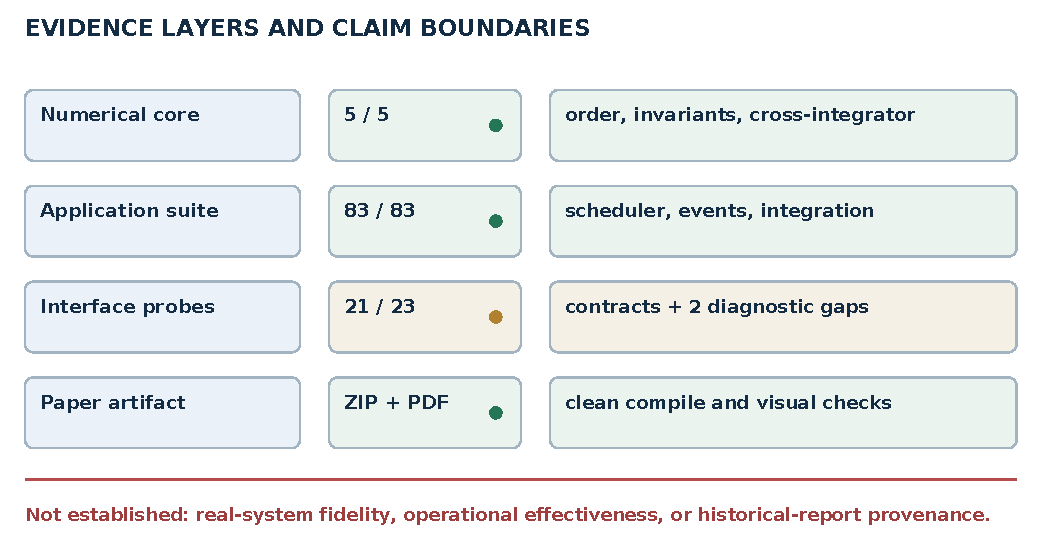
\includegraphics[width=\linewidth]{figures/verification_layers.pdf}
\caption{Layered verification and its claim boundary. Green cells denote fresh passing evidence; amber records diagnostic gaps rather than suppressing them. No software layer establishes real-system or operational validity.}
\label{fig:verification}
\end{figure}

\subsection{Application integration and artifact reproducibility}
The complete application test suite was executed from the simulation directory with pytest cache disabled and a JUnit report enabled. It reports \ApplicationTestsPassed passed and \ApplicationTestsFailed failed tests. Coverage includes configuration checks, state consistency, scheduler and event behavior, integrator verification, component interfaces, telemetry, and integration smoke paths. The count is an execution result from the retained XML record, not a static count of function definitions.

\begin{table}[H]
\caption{Fresh evidence used in this paper and the claims it can support.}
\label{tab:evidence}
\small
\begin{tabularx}{\linewidth}{@{}P{0.30\linewidth}P{0.20\linewidth}Y@{}}
\toprule
Evidence & Result & Supported scope \\
\midrule
Built-in numerical verification & \NumericalCases/\NumericalCases passed & Integrator order, invariants, projection, continuous-backend agreement \\
Application pytest suite & \ApplicationTestsPassed passed, \ApplicationTestsFailed failed & Implemented software behaviors exercised by the suite \\
Generic interface probes & 21/23 properties; 2 diagnostic gaps & Schema and Python telemetry boundary behavior \\
Allocation probes & 12/12 exact matches & Preallocated NumPy payload formula only \\
Independent source-ZIP build & Successful & Self-contained LaTeX/BibTeX/figure inputs \\
Historical report audit & \code{legacy\_unverified} & Absence of attributable original execution records \\
\bottomrule
\end{tabularx}
\end{table}

The paper build copies only referenced sources, compiles the manuscript, creates the arXiv ZIP, extracts it into a clean build directory, and recompiles using the bundled bibliography. PDF inspection checks page geometry, embedded fonts, selectable text, referenced figures, and source-archive consistency. Figure generators are retained and use no third-party artwork. These checks make the article artifact reproducible independently of the full simulator.

The evaluation has deliberate limits. Passing tests demonstrate behavior for their cases, not completeness. Numerical verification uses idealized problems and does not calibrate the physical models. The interface harness evaluates the Python path and does not prove equivalence of optional accelerated kernels. Deterministic seeded execution does not remove model-form uncertainty. Finally, three historical web reports lack matching original configuration, source, environment, and seed manifests; their numerical values are excluded rather than retrospectively attributed. The supported outcome is therefore a verified and inspectable simulation framework, not a validated real-world interception system or an operational performance claim.
\FloatBarrier

\section{Conclusion}
This paper reformulated \emph{Missile Intercept} as an end-to-end research framework whose principal contribution is explicit composition. The deterministic multi-rate closed-loop architecture fixes the sampled-data semantics and preserves them through RK4 stages and event refinement. The contract-driven state and telemetry interface connects named metadata to contiguous arrays while stating validation, ownership, capacity, and export behavior. The layered verification and traceability workflow links numerical checks, interface probes, application tests, seeded batches, and build artifacts to distinct claim boundaries.

In a fresh execution, all five numerical verification cases and all 83 application tests pass; 21 of 23 diagnostic interface properties are observed, with the two missing guards retained as limitations. The results support the implemented numerical and software contracts. They do not validate the fidelity of all physical models, establish optional-backend equivalence, or recover provenance for historical reports.

Future work will add finite checks at the two identified boundaries, test accelerated and pure-Python paths against the same contract suite, introduce configuration-schema versioning, and define public scenario and metric specifications suitable for a genuine benchmark. Physical validation should proceed separately through documented reference data and uncertainty analysis. This separation preserves the central lesson of the framework: timing, representation, and evidence must be explicit before simulated outcomes can be compared responsibly.

\section*{Software and Artifact Availability}
The anonymous paper folder contains LaTeX and BibTeX sources, original vector figures and their generator, machine-readable verification records, build and PDF checks, and a self-contained arXiv source archive. Author identities and affiliations remain intentionally anonymous. The source code is required to repeat the application tests; the arXiv archive is sufficient to reproduce the paper PDF.

\bibliographystyle{unsrtnat}
\bibliography{references}

\appendix
\section{Reproduction Commands and Evidence Map}
The fresh numerical and application checks can be repeated from the simulation directory:
\begin{lstlisting}
python verification.py --json ../arxiv-paper/evidence/numerical_verification.json
python -m pytest -q tests -p no:cacheprovider \
  --junitxml=../arxiv-paper/evidence/simulation_tests.xml
\end{lstlisting}
The paper artifacts can then be regenerated from \path{arxiv-paper}:
\begin{lstlisting}
python scripts/draw_figures.py
python scripts/build_paper.py --verify-zip
python scripts/check_pdf.py
\end{lstlisting}

The principal implementation-to-evidence links are: \path{main.py} and \path{integrator.py} for multi-rate and event semantics; \path{state_schema.py} and \path{telemetry.py} for data contracts; \path{verification.py} and \path{evidence/numerical_verification.json} for analytic cases; \path{tests/} and \path{evidence/simulation_tests.xml} for the fresh application suite; \path{evidence/software_probes.json} for isolated interface behavior; and \path{evidence/report_audit.json} for historical provenance status. All paths are relative to the source repository or paper folder as appropriate.

\end{document}
